% \documentclass[aps,prd,twocolumn,superscriptaddress,preprintnumbers,floatfix,nofootinbib]{revtex4-2}
\documentclass[reprint,amsmath,amssymb,aps,twocolumn]{aastex631}

\usepackage{showyourwork}
\usepackage{amsfonts,amssymb,amsmath}

\begin{document}

\title{Constraining gravitational wave amplitude birefringence with GWTC-3}

\author{Thomas C.K. Ng}
\email{thomas.ng@link.cuhk.edu.hk}
\affiliation{Department of Physics and Institute of Theoretical Physics, The Chinese University of Hong Kong, Shatin, Hong Kong}

\author{Maximiliano Isi}
\email{misi@flatironinstitute.org}
\affiliation{Center for Computational Astrophysics, Flatiron Institute, 162 5th Ave, New York, NY 10010, United States}

\author{Kaze W. K. Wong}
\email{kwong@flatironinstitute.org}
\affiliation{Center for Computational Astrophysics, Flatiron Institute, 162 5th Ave, New York, NY 10010, United States}

\author{Will M. Farr}
\email{wfarr@flatironinstitute.org}
\affiliation{Center for Computational Astrophysics, Flatiron Institute, 162 5th Ave, New York, NY 10010, United States}
\affiliation{Department of Physics and Astronomy, Stony Brook University, Stony Brook NY 11794, United States}

\date{\today}

\begin{abstract}

\end{abstract}

\section{Introduction}
\label{sec:Introduction}

% Motivation
Since Einstein proposed his theory of general relativity (GR), it was tested in a wide range of length scales.
After a century, we know that GR does not agree with quantum theories at some length scale.
To unify both theories, we need to study the possibility of different beyond-GR theories.
Some beyond-GR theories such as Chern-Simons gravity suggests that there is gravitational wave (GW) amplitude birefringence,
while GR predicts there is no birefringence.
GW amplitude birefringence is a property of space-time which consists of the enhancement of one GW polarization over the other during the propagation of the wave.
the local modification of the amplitude is small, but it grows with the number of cycles the GW is propagated.

% Previous studies
Previous studies have constrained amplitude birefringence by performing Bayesian inference.
In \citet{Maria_2021}, they considered the distribution of observed inclination of the GW events in GWTC-2, the second LIGO-Virgo catalog,
and use the distribution to constrain the amplitude birefringence effect with the assumption of frequency independence in GW amplitude birefringence.
In \citet{Yamada_2020} and \citet{Wang_2021}, they both modeled the waveform under birefringence effect with a simplify assumption and
performed Bayesian inference on the events in GWTC-1, the first LIGO-Virgo catalog.

% What's new?
In this paper, we used a birefringence model with higher order terms which include the frequency dependence of amplitude birefringence
to perform a more accurate parameter estimation (PE).
We also performed Bayesian inference on events in GWTC-3, the third LIGO-Virgo catalog.
We included all binary black hole merger events with smallest false alarm rate $\leq1\mathrm{yr^{-1}}$, which are listed in \citet{GWTC_3_population}.

% Section guide
In Sec.~\ref{sec:Method}, we describe the modification we made to the waveform model, and mention the configuration we used in the PE.
In Sec.~\ref{sec:Results}, we show the combined result of the PE, and present the constrain on the GW amplitude birefringence we obtained.
In Sec.~\ref{sec:Discussion}, we discuss the limitation of this study, and provide suggestions for future studies.

\section{Method}
\label{sec:Method}

% Waveform modification
GW consist of two linear polarizations (i.e. $+$ and $\times$) similar to electromagnetic waves,
which could be transformed into two circular polarizations (i.e. left-handed and right-handed) by
\begin{equation}
    h_{\mathrm{L/R}} = \frac{h_+ \pm i h_\times}{\sqrt{2}}\,,
\end{equation}
where $h_{\mathrm{L/R}}$ are the Fourier amplitude of the left-handed and right-handed polarization of the waveform,
$h_+$ and $h_\times$ are the Fourier amplitude of the plus and cross polarization of the waveform.
According to \textbf{[modification reference]}, we modified the waveform model by
\begin{equation}
    h_\mathrm{L/R}^{\mathrm{br}}=
    h_\mathrm{L/R}^{\mathrm{GR}}\times
    \exp\left(\pm\kappa\frac{d_C}{1\mathrm{Gpc}}\frac{f}{100\mathrm{Hz}}\right)\,,
\end{equation}
where $h_\mathrm{L/R}^{\mathrm{br}}$ is the Fourier amplitude of the modified waveform with amplitude birefringence,
$h_\mathrm{L/R}^{\mathrm{GR}}$ is the Fourier amplitude of the waveform at the source,
$\kappa$ is the dimensionless opacity parameter that represent the strength of the birefringence,
$d_C$ is the comoving distance to the source, and $f$ is the Fourier frequency of the waveform.
We assume GWs are generated by the binary as GR predicts, as the modification at the source is small before the effect accumulate during the propagation.
As the GWs propagate, the effect of birefringence will be built up with the number of cycles which depends on the distance traveled and the frequency of the GWs.

% Effect on inclination PE
This modification changes the ratio of the left-handed and right-handed polarization of the waveform,
which affects the PE on the inclination as well.
In GR, the amplitude ratio of the left-handed and right-handed polarizations only depends on the inclination for a nonprecessing binary.
The relationship between the amplitude ratio and the inclination is
\begin{equation}
    \frac{h_\mathrm{L}}{h_\mathrm{R}}=\left(\frac{1-\cos\iota}{1+\cos\iota}\right)^2\,,
\end{equation}
where $h_\mathrm{L}$ and $h_\mathrm{R}$ are the Fourier amplitude of left-handed and right-handed polarizations of the GWs
and $\iota$ is the inclination, the angle between our line of sight and the orbital angular momentum of the binary.
PE on $\iota$ takes the amplitude ratio into account. Therefore, the PE on $\iota$ depends on the amplitude ratio.

With the modification we implemented, the amplitude ratio of the left-handed and right-handed polarizations becomes 
\begin{equation}
    \frac{h_\mathrm{L_{obs}}}{h_\mathrm{R_{obs}}}=\frac{\left(1-\cos\iota\right)^2}{\left(1+\cos\iota\right)^2}\exp\left({2\kappa\frac{d_C}{1\mathrm{Gpc}}\frac{f}{100\mathrm{Hz}}}\right)\,,
\end{equation}
where $h_\mathrm{L_{obs}}$ and $h_\mathrm{R_{obs}}$ are the observed Fourier amplitude of left-handed and right-handed polarizations of the GWs.
As the amplitude ratio does not only depends on $iota$ with this modification, but also $\kappa$ and $d_C$,
the PE on $\iota$ and $d_C$ are affected. Note that GR is recovered if $\kappa$ is $0$.

For some previous studies on the birefringence property such as \citet{Maria_2021}, they assume the effect of birefringence is independent of the frequency,
which is a zeroth-order approximation of the birefringence model in Chern-Simons gravity.
This would create a degeneracy between kappa and iota, as they can affect the amplitude ratio in the same way.
To reconstruct the amplitude ratio from the interferometer data, an $\iota$ representing a more face-off inspiral can pair with a positive $\kappa$,
or an $\iota$ representing a more face-on inspiral with a negative $\kappa$.
As a result, many pairs of $\iota$ and $\kappa$ can be plausible with the frequency independence.

In contrast, We included the frequency dependence in the modification, which is a first-order approximation of the birefringence model.
This frequency dependence provides stronger enhancement or suppression from the birefringence to high frequency components of the GW, and visa versa.
Also, the frequency dependence can break the degeneracy between kappa and iota,
as this would make the effect of the birefringence affect the amplitude ratio differently compared to iota.
To illustrate the frequency dependence of amplitude birefringence,
the observed amplitudes of two polarizations of a simulated GW signal are shown in figure \ref{fig:birefringence}.

\begin{figure}[h]
    \script{birefringence.py}
    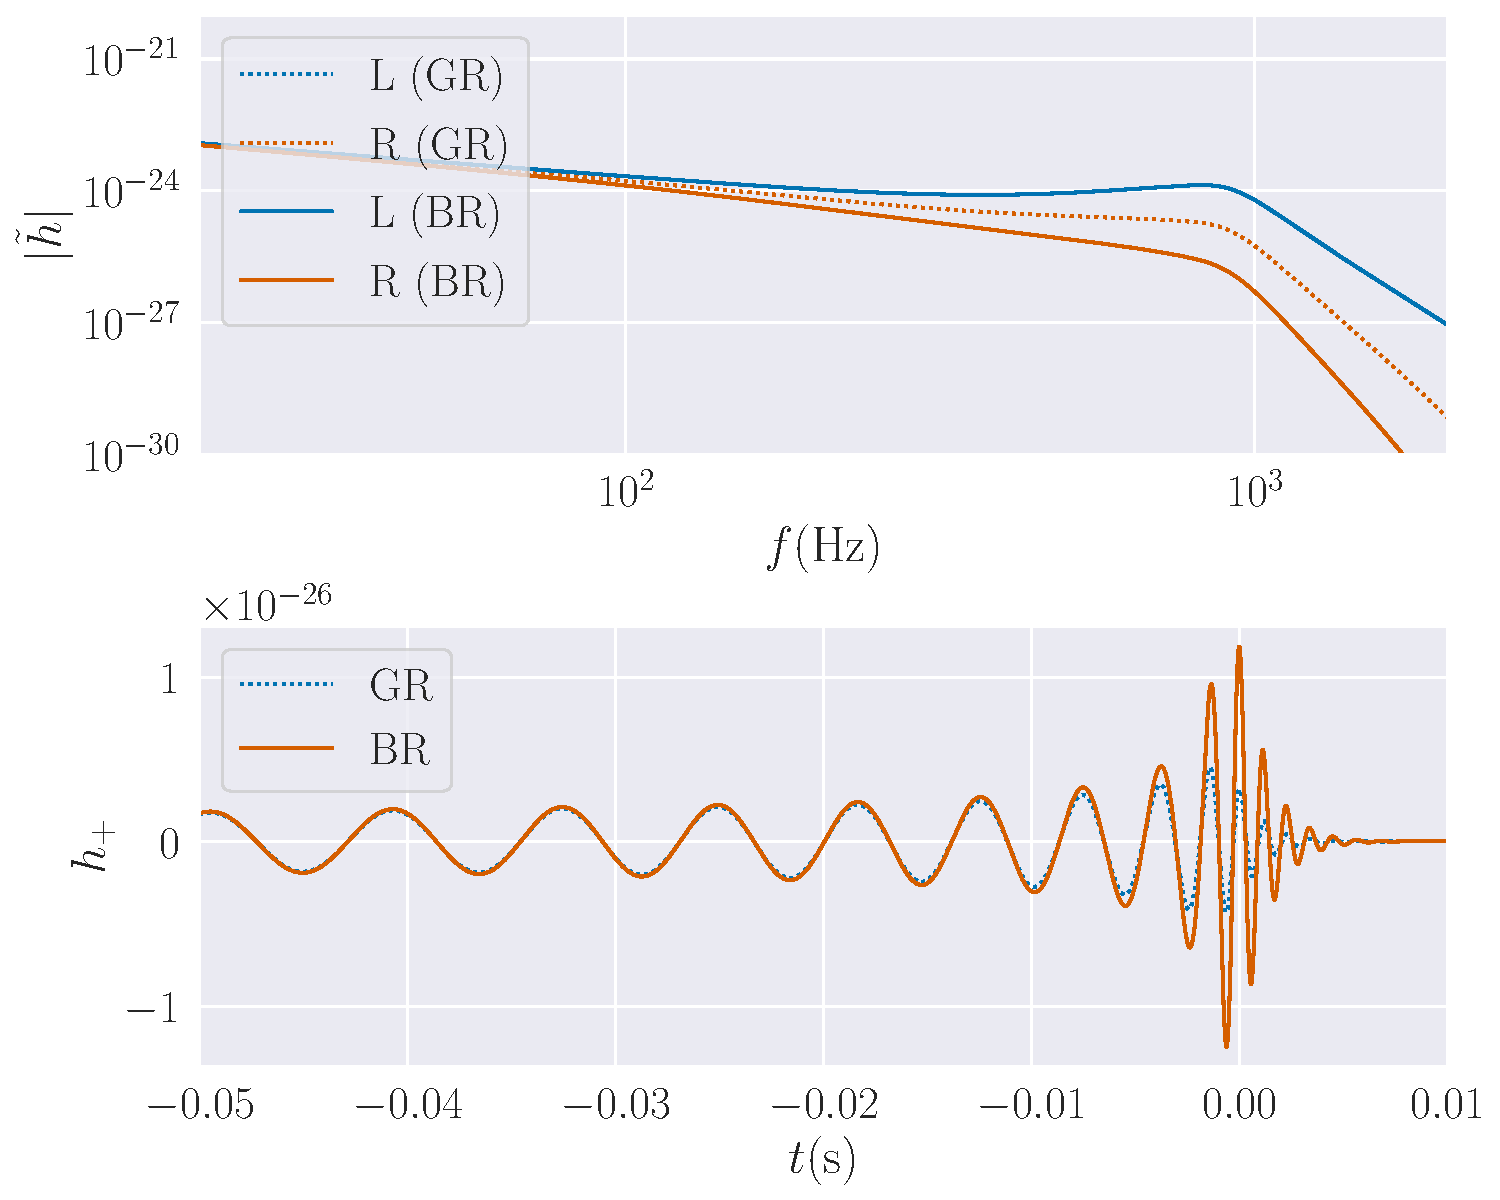
\includegraphics[width=\columnwidth]{figures/birefringence.pdf}
    \caption{
        The observed Fourier amplitude of two polarizations of an simulated GW signal with and without birefringence.
        The amplitudes as GR predicts are shown in dotted lines with blue and orange colors representing the left-handed and right-handed polarizations.
        The amplitudes with birefringence are shown in solid lines with blue and orange colors representing the left-handed and right-handed polarizations.
        This shows the effect of amplitude birefringence with the frequency dependence.
    }
    \label{fig:birefringence}
\end{figure}

% Parameter estimation
To constrain $\kappa$, we perform PE with data from the third LIGO-Virgo catalog \citep{GWTC-2.1, GWTC-3}, GWTC-3, using Bilby,
a Bayesian toolkit for GW data analysis which is able to calculate posteriors of GW parameters based on interferometer data
and priors for the parameters in question \citep{Bilby}. 
We set the prior on $\kappa$ to a uniform distribution between $-1$ and $1$
\footnote{For \textbf{[some events]}, a uniform distribution between $-0.5$ and $0.5$ was used instead. This does not affect the posterior distribution.},
and perform PE using the modified waveforms.
In both case, we use the same PE configuration as in \citet{GWTC-2.1, GWTC-3} for each individual events, excluding the calibration of the detectors.
We also perform test to check if the PE could recover the PE done by LIGO in \citet{GWTC-2.1, GWTC-3}.
We set the prior on $\kappa$ to be a $\delta$ function at $0$, which is the same as using GR.
These control tests result can be found in the data release.

\section{Results}
\label{sec:Results}

\subsection{Result on GWTC-3}
% Combined plot

% How to calculate the combined posterior

% Constraint on $\kappa$

% Violin plot

% Trend (mass & distance)

% Constraining power

% Case study

% Case 1: GW150914
\subsection{Result on GW150914}

\begin{figure}[h]
    \script{GW150914_corner.py}
    \includegraphics[width=\columnwidth]{figures/GW150914_corner.pdf}
    \caption{
        The posterior of $\kappa$, luminosity distance $d_L$ and $\cos{\iota}$ for GW150914.
    The three colors in the plot are the PE with GR done by LIGO without cosmological reweighing \citep{GWTC-2.1, GWTC-3},
    the PE done by us with the frequency independent birefringence and the frequency dependent birefringence respectively.
    Note that there is no posterior of $\kappa$ for the PE from LIGO, as the LIGO PE is based on GR,
    which does not suggest GW amplitude birefringence. The plot shows that frequency independent birefringence create a degeneracy between $\kappa$ and $\iota$,
    while the frequency dependent birefringence can break it.
    }
    \label{fig:GW150914_corner}
\end{figure}

Consider GW150914, the first GW detected by LIGO. In figure \ref{fig:GW150914_corner}, we show the posteriors of the parameters of GW150914.
With the frequency independent birefringence model, the posteriors for $\cos\iota$ look different from the posteriors assuming GR.
This is because, for a nonprecessing system, there is a degeneracy between $\kappa$ and $\iota$ if the frequency dependence is not included.
To reconstruct the amplitude ratio from the interferometer data, an $\iota$ representing a more face-off inspiral can pair with a positive $\kappa$,
or an $\iota$ representing a more face-on inspiral with a negative $\kappa$.
As a result,many pairs of $\iota$ and $\kappa$ can be plausible with the frequency independence.

On the other hand, with the frequency-dependent birefringence model, the posterior looks similar to the GR posterior.
This is because the degeneracy was broken by the frequency dependence, as the effect of the birefringence will be different from the one of changing $\iota$.
In this case, the posteriors can recover the GR distributions for the binary parameters,
and the most probable value of $\kappa$ is close to $0$, which means the birefringence is weak or absent, and GR can be recovered.

\section{Discussion}
\label{sec:Discussion}

% Reasons for special events

% BNS

% Higher order terms

% More observations with higher SNR


\section{Acknowledgements}
\label{sec:Acknowledgements}



\bibliography{bib}

\end{document}
